\documentclass[conference]{IEEEtran}
\IEEEoverridecommandlockouts
% The preceding line is only needed to identify funding in the first footnote. If that is unneeded, please comment it out.
\usepackage{cite}
\usepackage{amsmath,amssymb,amsfonts}
\usepackage{algorithmic}
\usepackage{graphicx}
\usepackage{textcomp}
%\usepackage{xcolor}
\usepackage[utf8]{inputenc}
\usepackage{hyperref}
\hypersetup{hidelinks}
\usepackage{float}
\usepackage{placeins}
\usepackage{tabularx}
\usepackage{setspace}


\def\BibTeX{{\rm B\kern-.05em{\sc i\kern-.025em b}\kern-.08em
    T\kern-.1667em\lower.7ex\hbox{E}\kern-.125emX}}

\usepackage[letterpaper, top=1in, bottom=1.05in, left=0.68in, right=0.68in]{geometry}

\begin{document}

\title{AI- Generated Text Detection Based on Transfomer Model}

%====================================================================

\author{
\begin{tabular}{cc}

\begin{minipage}[t]{0.45\textwidth}
    \centering
    \text{1\textsuperscript{st} Ho Giang Long Nguyen} \\
    \textit{Ho Chi Minh City Open University, Vietnam} \\
    2351010115long@ou.edu.vn
\end{minipage}
&
\begin{minipage}[t]{0.45\textwidth}
    \centering
    \text{2\textsuperscript{nd} Thien Ho Huong*} \\
    \textit{Ho Chi Minh City Open University, Vietnam} \\
    thien.hh@ou.edu.vn
\end{minipage}

\end{tabular}
}

\maketitle

\begin{abstract}
Phan nay la doan abstract, se viet cuoi cung sau khi hoan thanh cac buoc
\end{abstract}

\begin{IEEEkeywords}
AI Generated text detection, Human-Generated text, Transformer models, Hybrid Deep Learning, Phishing Detection.
\end{IEEEkeywords}

\section{Introduction}



The main contributions of this research are as follows:

\begin{itemize}
\item Dong gop thu nha.

\item Dong gop thu hai.

\item Dong gop thu ba.
\end{itemize}

\section{Related Works}
Methods have evolved through generations of approaches: hand-crafted features, deep learning models applied directly to URL text \cite{hung}, and, more recently, multi-view models that learn from several URL representations simultaneously. While each generation addresses the weaknesses of its predecessor, it introduces its own trade-offs.

Initially, researchers trained classifiers using features manually engineered from URL strings, DNS resolution data, Whois records, and page content. For instance, Mahammad Rafi et al. \cite{Mahammad} extracted features based on URL length, character distribution, and segment organization to detect spoofed login pages. Although they demonstrated that URL structure provides effective signals for phishing detection, their work also exposed the limitations of hard-coded rules: attackers can easily evade detection once they uncover the target features. In the study \cite{Bu}, Bu et al. combined CNN-based feature extraction with ensemble learning to improve robustness, aggregating predictions across multiple models under the assumption that individual errors can be corrected by the ensemble. However, like other early approaches, this method still relied on human-engineered features, leaving it vulnerable to subtle adversarial modifications. Overall, feature-based methods rely on hand-crafted heuristics that fail to adapt as attacker strategies evolve, while feature creation itself demands significant domain expertise. These inherent limitations of feature engineering have driven the shift toward automatic pattern learning.



\section{Methodology}
This study proposes a character-level hybrid deep learning approach for phishing URL detection. The overall workflow, illustrated in Fig.\ref{fig:overall}, includes data collection and pre-processing, model training and threshold tuning, evaluation, and baseline comparison.


\begin{figure}
    \centering
    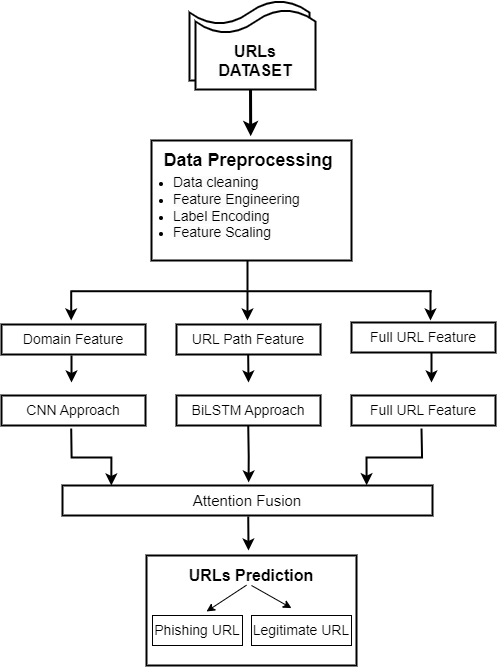
\includegraphics[width=1\linewidth]{overal.png}
    \caption{Overall of the proposed Hybrid Model}
    \label{fig:overall}
\end{figure}

\subsection{Data preparation and Pre-processing}
\subsubsection{\textbf{Dataset}}
A binary URL classification dataset was constructed by crawling two continuously updated phishing intelligence feeds: PhishTank \cite{phishtank} and OpenPhish \cite{openphish}. Phishing URLs were collected during June--July 2025. Benign URLs were sourced from top-ranked domain lists and verified clean URL corpora. After preprocessing, the final dataset comprises 464,133 URLs: 345,702 benign (74.5\%) and 118,431 phishing (25.5\%).

\subsubsection{\textbf{Pre-processing}}
Four sequential steps are applied to prepare raw URL strings for model injection.

\begin{itemize}
\item First, rows with missing URL or label values are discarded, and duplicate URLs are removed. URLs not beginning with protocol http or https, or URLs lengths outside the range 10 and 2,000 are excluded as malformed.
\item Second, each URL is decomposed into three structural components-domain, path, and full URL string which serve as dedicated inputs to the three encoder branches.
\item Third, a character-level vocabulary is constructed from the training set (lowercase), yielding 147 tokens including special tokens \texttt{<PAD>} (index 0) and \texttt{<UNK>} (index 1). Each component sequence is integer-encoded and truncated or zero-padded to its component-specific maximum length (domain: 45, path: 155, full URL: 180), set at the 99th percentile to limit truncation to under 1\% of samples.
\item Finally, encoded sequences are stored as 16-bit arrays loaded via memory-mapped I/O to handle the large dataset efficiently.
\end{itemize}


The dataset is split into training (70\%), validation (15\%), and test (15\%) partitions using a stratified split with a random seed of 42 to preserve the class distribution across all subsets, as summarized in Table \ref{tab:dataset_partition}.

\begin{table}[htbp]
\caption{Dataset Partition distribution }
\label{tab:dataset_partition}
\centering
\begin{tabular}{llll}
\hline
\textbf{Partition} & \textbf{Total} & \textbf{Benign} & \textbf{Phishing} \\ \hline
Train & 324,893 & 241,991 & 82,902 \\
Validation & 69,620 & 51,855 & 17,765 \\
Test & 69,620 & 51,856 & 17,764 \\ \hline
\end{tabular}
\end{table}

\subsection{Models Architecture}
To take advantage of the different structures within a URL, we propose a hybrid character-level model with three approaches and attention-based fusion, which we call \texttt{Hybrid Model}. The attention mechanism is commonly used in text classification to improve feature extraction \cite{zhou} \cite{Yan}. It helps the model focus on the most relevant words while retaining important information from the text.



%\begin{figure}[H]
%    \centering
%    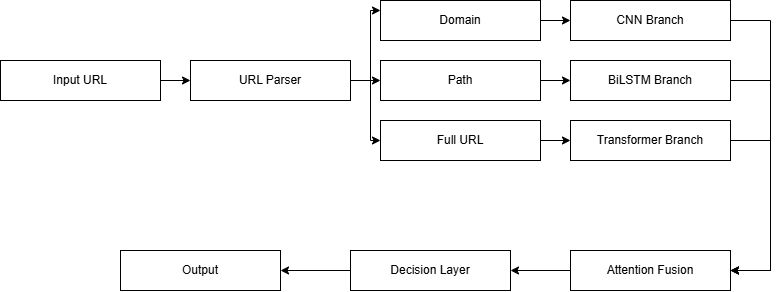
\includegraphics[width=1\linewidth]{Overall_1.png}
%    \caption{Overall architecture of PhishingHybridModel.}
%    \label{fig:architecture}
%\end{figure}


    \item \textbf{Path Branch-Bidirectional LSTM:} The Path Branch employs a Character Encoder (Embedding Layer) that maps the input path sequence, with shape $[\text{Batch} \times 155]$, into 64-dimensional character embeddings. This sequence is then fed into a 2-layer Bidirectional LSTM with a hidden size of 64 per direction (128 combined), producing Hidden States of shape $[\text{Batch} \times 155 \times 128]$. An Attention Layer then computes a weighted sum over the time-step dimension, using a linear projection ($128 \rightarrow 1$) followed by Softmax, to emphasize the most informative character positions. The attended representation is passed through a Fully Connected layer ($128 \rightarrow 128$) to produce the final path branch embedding $f_{\text{path}}$ (Output: $[\text{Batch} \times 128]$).

%    \begin{figure}[H]
%        \centering
%        \includegraphics[width=1\linewidth]{BiLSTM_Branch.png}
%        \caption{Path Branch-Bidirectional LSTM Architecture}
%        \label{fig:bilstm_branch}
%    \end{figure}

    \item \textbf{Full-URL Branch-Transformer Encoder:} The Full URL Branch employs a Character Encoder (Position Encoder) that adds learnable positional embeddings, $E_{\text{pos}}$, to the character embeddings of the input sequence, with shape $[\text{Batch} \times 180]$, injecting position information adapted to URL character distributions rather than using fixed sinusoidal encodings. The combined representation is then processed by a Transformer Layer configured with 8 attention heads and an FFN dimension of 256 ($d_{\text{model}} = 64$, $\text{dropout} = 0.3$), with a \texttt{<PAD>}-derived key padding mask used to prevent attention over padding tokens. This produces an Encoded Sequence of shape $[\text{Batch} \times 180 \times 64]$, which is aggregated by a Pooling Layer through mean pooling over non-padded positions. A Fully Connected layer ($64 \rightarrow 128$) then maps the pooled vector to the final full-URL branch embedding $f_{\text{url}}$ (Output: $[\text{Batch} \times 128]$).
    
%    \begin{figure}[H]
%        \centering
%        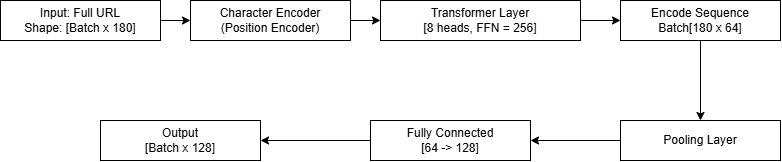
\includegraphics[width=1\linewidth]{Transformer_Branch.png}
%        \caption{Full-URL Branch - Transformer Encoder Architecture}
%        \label{fig:transformer_branch}
%    \end{figure}

    \item \textbf{Attention-Based Late Fusion and Decision Layer:} As depicted in Fig. \ref{fig:attention_fusion}, the three branch embeddings – $f_{\text{domain}}$, $f_{\text{path}}$, and $f_{\text{url}}$ – are aggregated through a two-layer attention network. Stacking all embeddings, an attention layer is used to compute a content-aware weight for each branch. Computing the weighted sum gives a fused representation. As these weights are content-dependent, the network is capable of dynamically focusing on the most discriminative URL feature based on the input, thus avoiding the risk of a benign domain signal overshadowing a phishing path signal, a major drawback of static weights \cite{Maneriker}. The fused embedding is then fed to the decision layer, which consists of a fully connected layer ($128 \rightarrow 64$) with ReLU activation and dropout rate 0.3, and a linear layer ($64 \rightarrow 2$).


%==============================================================================================================%


\subsection{Model Evaluation Metrics}
In order to measure the performance of the phishing URL detection models, the following classification performance indicators were used: Accuracy, Precision, Recall, F1-Score, Macro F1-Score, AUC-ROC, False Negatives (FN), False Positives (FP). 

\textbf{Accuracy}  is the indicator that measures the general ability of the model to predict the correct class for the URL. The metric is calculated as a ratio of correctly predicted samples to the total number of samples.

%\begin{equation}
%\text{Accuracy} = \frac{\text{TP} + \text{TN}}{\text{TP} + \text{TN} + \text{FP} + \text{FN}}
%\end{equation}

\textbf{Precision} represents the percentage of correctly identified phishing URLs out of all the URLs that have been classified as phishing URLs.
%\begin{equation}
%\text{Precision} = \frac{\text{TP}}{\text{TP} + \text{FP}}
%\end{equation}

\textbf{Recall} (Sensitivity) represents the ability of the classifier to identify the actual phishing URLs.
%\begin{equation}
%\text{Recall} = \frac{\text{TP}}{\text{TP} + \text{FN}}
%\end{equation}

\textbf{F1-Score} represents the harmonic mean between Precision and Recall.
%\begin{equation}
%\text{F1-Score} = 2 \times \frac{\text{Precision} \times \text{Recall}}{\text{Precision} + %\text{Recall}}
%\end{equation}

\textbf{Macro F1-Score}  is the main metric used in this study. It calculates the arithmetic average of the F1-scores for each class, irrespective of the classes.
%\begin{equation}
%\text{Macro F1} = \frac{1}{C} \sum_{c=1}^{C} \text{F1}_c = \frac{\text{F1}_{\text{phishing}} + \text{F1}_{\text{legitimate}}}{2}
%\end{equation}

\textbf{AUC-ROC} represents the discriminative ability of the classifier without considering any threshold.
%\begin{equation}
%\text{AUC-ROC} = \int_{0}^{1} \text{TPR}\left(\text{FPR}^{-1}(t)\right)\, dt
%\end{equation}
%where TPR and FPR are defined as:
%\begin{equation}
%\text{TPR} = \frac{\text{TP}}{\text{TP} + \text{FN}}, \quad \text{FPR} = \frac{\text{FP}}%{\text{FP} + \text{TN}}
%\end{equation}



%==============================================================================================================%
\section{Experimental Setup}
To assess the effectiveness of the proposed hybrid deep learning architecture in phishing URL detection, we trained and evaluated five distinct model configurations: the proposed Hybrid Model and four single-branch baselines includes CNN, BiLSTM, Transformer, and a Simple Concat. Each model was trained independently on the same dataset partitions with consistent hardware and software environments (PyTorch 2.1.0+cu121, NVIDIA Tesla T4 GPU), enabling fair comparison.


\textbf{CNN Model:} 

\textbf{BiLSTM Model with Attention Mechanism:} 

\textbf{Transformer Model:} 

\textbf{Proposed Hybrid Model:} The proposed triple-branch hybrid model was trained for 30 epochs with a batch size of 256. A Weighted Cross-Entropy loss with inverse-frequency class weights was used to address the $74.5\% / 25.5\%$ class imbalance


Detailed hyperparameter settings for the proposed model are listed in Table \ref{tab:hyperparameters}.

\begin{table}[htbp]
\caption{Model Training Hyperparameters}
\label{tab:hyperparameters}
\centering
\begin{tabular}{lc}
\hline
\textbf{Hyperparameter} & \textbf{Value} \\ \hline
Optimizer & AdamW \\
Learning rate & $1 \times 10^{-3}$ \\
Gradient clip norm & 1.0 \\
Batch size & 256 \\
Epochs & 30 \\
Random seed & 42 \\ \hline
\end{tabular}
\end{table}


\section{Results and Discussion}
In this section, we present the performance comparison of the Hybrid Model against four different baseline models 

As can be seen from Table \ref {tab:test_performance}, the Hybrid Model proposed 

\begin{table}[htbp]
\caption{Performance of Approaches on the Test Set ($n = 69,620$)}
\label{tab:test_performance}
\centering
\resizebox{\linewidth}{!}{%
\begin{tabular}{lccccc}
\hline
\textbf{Model} & \textbf{Macro F1} & \textbf{AUC-ROC} & \textbf{Precision} & \textbf{Recall} & \textbf{Params} \\ \hline
CNN & 99.50 & 99.90 & 98.16 & 99.17 & 83,522\\
BiLSTM & 85.62 & 94.69 & 68.97 & 96.23 & 84,354 \\
Transformer & 99.37 & 99.88 & 97.21 & 99.21 & 75,202\\
Simple Concat & 99.14 & 99.96 & 98.45 & 98.44 & 292,226 \\
\textbf{Proposed} & 99.44 & \textbf{99.97} & \textbf{98.92} & 99.10 & \textbf{280,003} \\ \hline
\end{tabular}%
}
\end{table}


\begin{figure}
    \centering
    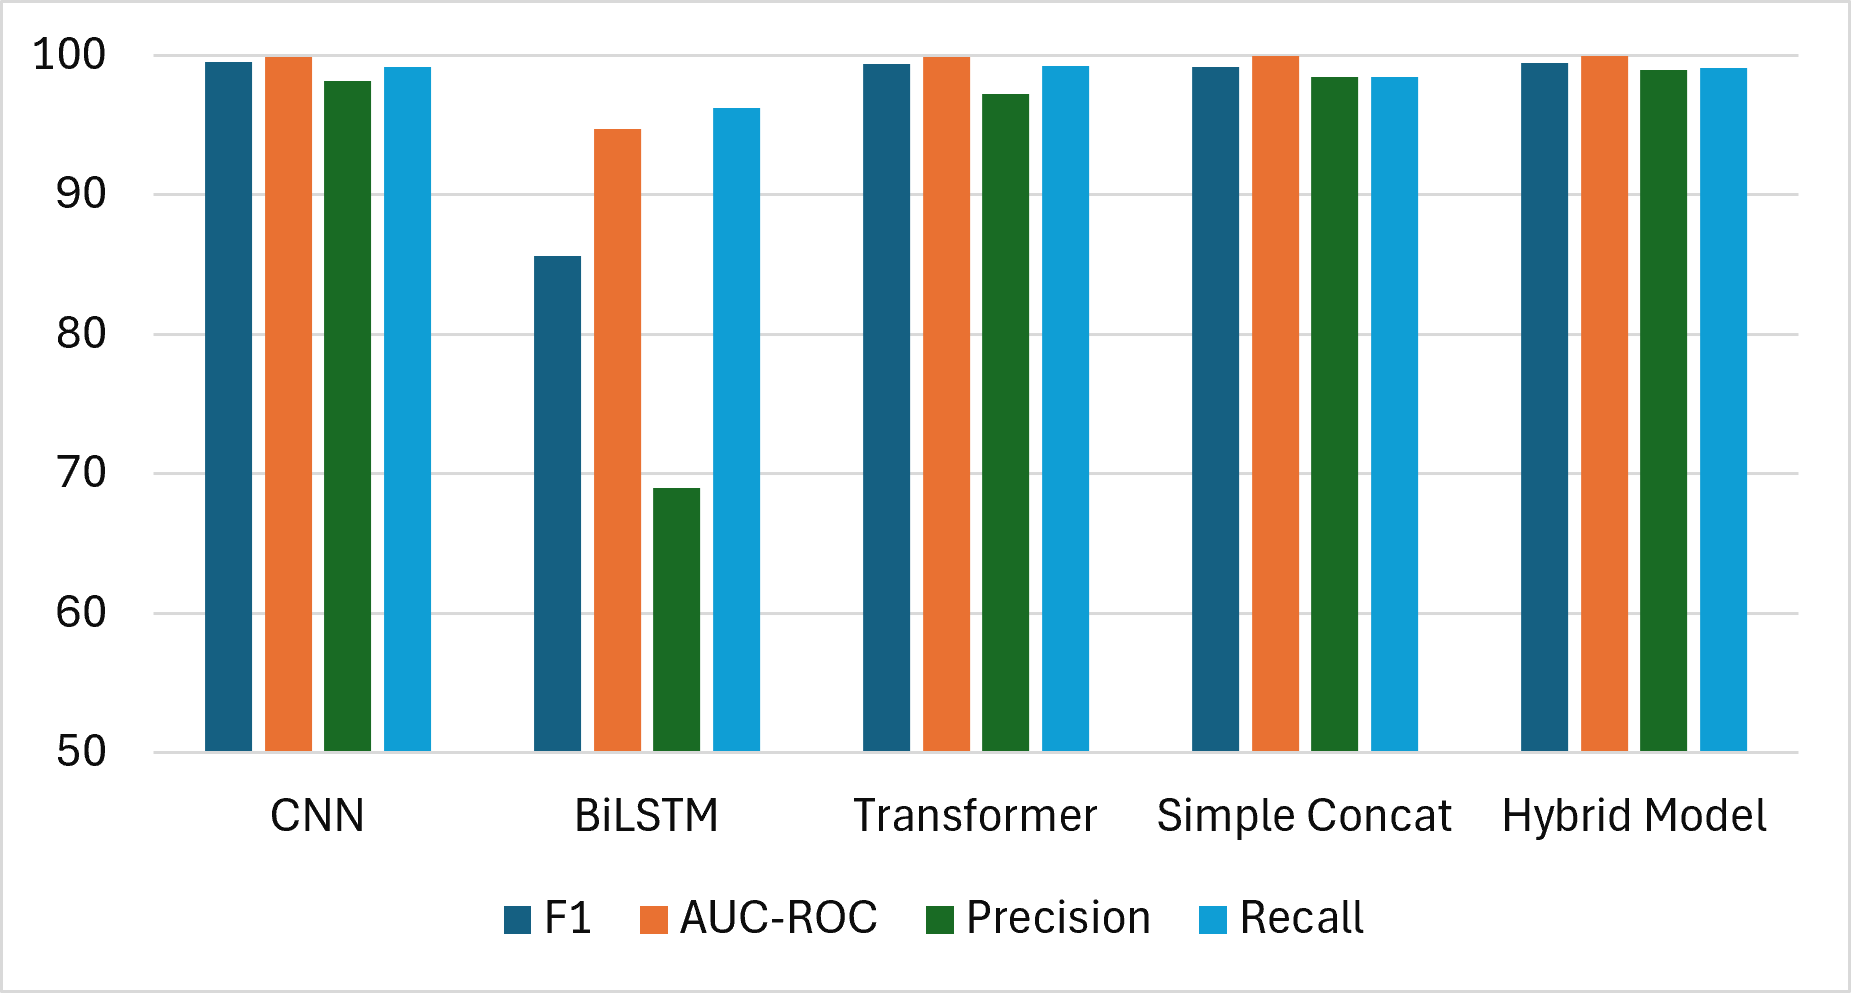
\includegraphics[width=1\linewidth]{result_chart.png}
    \caption{Models performance comparison}
    \label{fig:result_chart}
\end{figure}

To better understand the model's behavior at the decision threshold, Table \ref{tab:confusion_matrix} presents the confusion matrix of the Hybrid Model on the test set. Out of the total of 69,620 test instances, the model was able to correctly identify 51,717 legitimate URLs and 17,605 phishing URLs, while committing 159 false negatives and 139 false positives.

\begin{table}[htbp]
\caption{Proposed Model Confusion Matrix}
\label{tab:confusion_matrix}
\centering
\begin{tabular}{lcc}
\hline
 & \textbf{Legitimate (0)} & \textbf{Phishing (1)} \\ \hline
\textbf{Legitimate (0)} & 51,717 (TN) & 139 (FP) \\
\textbf{Phishing (1)} & 159 (FN) & 17,605 (TP) \\ \hline
\end{tabular}
\end{table}

For comparison across different models, Table \ref{tab:confusion_matrix_summary} shows the corresponding confusion matrix entries. First of all, it can be seen that the results for BiLSTM are substantially worse than for the hybrid approach since BiLSTM leads to False Positives = 7846 (FPR = 15.13\%), which means that every sixth legitimate URL would have been blocked. By introducing the domain-aware CNN branch, $\texttt{Hybrid Model}$ reduces the FPR significantly (FPR = 0.268\%).

\begin{table}[htbp]
\caption{Confusion Matrix Summary - All Models (Test Set)}
\label{tab:confusion_matrix_summary}
\centering
\resizebox{\linewidth}{!}{%
\begin{tabular}{lcccccc}
\hline
\textbf{Model} & \textbf{TP} & \textbf{TN} & \textbf{FP} & \textbf{FN} & \textbf{Recall} & \textbf{FPR} \\ \hline
CNN & 17,616 & 51,742 & 114 & 148 & 99.17\% & 0.220\% \\
BiLSTM & 17,093 & 44,010 & 7,846 & 671 & 96.23\% & 15.13\% \\
Transformer & 17,623 & 51,662 & 194 & 141 & 99.21\% & 0.374\% \\
Simple Concat & 17,486 & 51,681 & 175 & 278 & 98.44\% & 0.338\% \\
\textbf{Proposed} & \textbf{17,605} & \textbf{51,717} & \textbf{139} & \textbf{159} & \textbf{99.10\%} & \textbf{0.268\%} \\ \hline
\end{tabular}%
}
\end{table}

The results show that URL structural decomposition is necessary but not sufficient for reliable phishing detection. BiLSTM model performs poorly because path-only analysis cannot distinguish a benign path on a trusted domain from a similarly structured malicious one without domain-level information. CNN performs strongly by capturing domain-level patterns such as typosquatting, though its lower AUC-ROC than Hybrid Model shows less separation across decision thresholds. Simple Concat method, despite using the same encoders as Hybrid Model, underperforms because fixed concatenation allows one branch to suppress weaker but important signals from another.


%\begin{table}[htbp]
%\caption{Ablation Study Results}
%\label{tab:ablation_study}
%\centering
%\resizebox{\linewidth}{!}{%
%\begin{tabular}{l|c|c|c|c|c|c}
%\hline
%\textbf{Model} & \textbf{Val Macro F1} & \textbf{Val AUC} & \textbf{Test Macro F1} & \textbf{Test AUC} & \textbf{FN} & \textbf{FP} \\ \hline

%NoCNN & 0.9906 & 0.9980 & 0.9901 & 0.9982 & 289 & 234 \\
%NoLSTM & \textbf{0.9962} & 0.9995 & 0.9956 & 0.9996 & 141 & 91 \\
%NoTransformer & \textbf{0.9962} & \textbf{0.9996} & \textbf{0.9957} & 0.9996 & \textbf{136} & \textbf{90} \\
%AvgFusion & 0.9903 & 0.9994 & 0.9893 & 0.9994 & 366 & 197 \\ \hline
%\textbf{Proposed} & 0.9949 & \textbf{0.9996} & 0.9944 & \textbf{0.9997} & 159 & 139 \\
%\end{tabular}%
%}
%\end{table}


\section{Conclusion}
This paper presented Hybrid Model, which splits each URL into domain, path, and full URL, processes each part with a matched network (a multi-scale 1D-CNN for the domain, a Bidirectional LSTM


The model is also relatively lightweight, with only 280,003 parameters and about 58 minutes of training time on a single GPU, making it potentially suitable for fast applications such as browser extensions, pending further real-world testing. This work has some limitations, including binary-only classification, a short two-month data collection period, no explicit handling of techniques like Punycode encoding, and reliance on URL text alone without webpage content; future work could test the model on longer-term data, extend it to classify attack types, and incorporate webpage-content signals when higher accuracy is needed. Overall, this study suggests that decomposing a URL into structural components and combining them via learned attention can be a useful approach to phishing detection, within the scope of the dataset and experiments presented here.

\begin{thebibliography}{11}


\bibitem{Wicaksana}
H. S. Wicaksana, U. Ependi, and A. Muzakir, “URL-Based Phishing DetectFion Using a BERT-LSTM Model,” journalisi, vol. 8, no. 1, pp. 1344–1367, Apr. 2026.

\bibitem{report}
Anti-Phishing Working Group, Phishing attack trends report 1st 2026, https://docs.apwg.org/reports/apwg\_trends\_report\_q1\_2026.pdf, May. 2026, Online accessed:  Aug. 2026.

\bibitem{Aljaidi}
M. Aljaidi et al., “Cybersecurity Threats in the Era of AI: Detection of Phishing Domains Through Classification Rules,” in 2023 2nd International Engineering Conference on Electrical, Energy, and Artificial Intelligence (EICEEAI), Zarqa, Jordan: IEEE, pp. 1–6, Dec. 2023.

\bibitem{Mahammad}
D. Mahammad Rafi et al., “Advanced detection of phishing URLs: An empirical study through login URL pattern analysis,” JIOS, vol. 46, no. 2, pp. 467–483, 2025.


\bibitem{Maneriker}
P. Maneriker, J. W. Stokes, E. G. Lazo, D. Carutasu, F. Tajaddodianfar, and A. Gururajan, “URLTran: Improving Phishing URL Detection Using Transformers,” Aug. 27, 2021.

\bibitem{Bu}
S.-J. Bu and H.-J. Kim, “Ensemble Learning of Deep URL Features based on Convolutional Neural Network for Phishing Attack Detection,” Adv. sci. technol. eng. syst. j., vol. 6, no. 5, pp. 291–296, Oct. 2021.
\bibitem{Aslam}
S. Aslam, H. Aslam, A. Manzoor, H. Chen, and A. Rasool, “AntiPhishStack: LSTM-Based Stacked Generalization Model for Optimized Phishing URL Detection,” Symmetry, vol. 16, no. 2, p. 248, Feb. 2024.

\bibitem{Vulfin}
A. Vulfin, A. Sulavko, V. Vasiliev, A. Minko, A. Kirillova, and A. Samotuga, “A Multimodal Phishing Website Detection System Using Explainable Artificial Intelligence Technologies,” MAKE, vol. 8, no. 1, p. 11, Jan. 2026.

\bibitem{Wang}
Y. Wang, W. Ma, H. Xu, Y. Liu, and P. Yin, “A Lightweight Multi-View Learning Approach for Phishing Attack Detection Using Transformer with Mixture of Experts,” Applied Sciences, vol. 13, no. 13, p. 7429, Jun. 2023.

\bibitem{hung}
H. D. Nguyen and T. H. Huong, “Phishing Website Detection Using Deep Learning Based on URL Feature Extraction,” in 2025 1st International Conference on Emerging Trends in Information Systems and Informatics (ICETISI), Jakarta, Indonesia: IEEE, pp. 1–7, Dec. 2025.

\bibitem{Le}
H. Le, Q. Pham, D. Sahoo, and S. C. H. Hoi, “URLNet: Learning a URL Representation with Deep Learning for Malicious URL Detection,” Mar. 02, 2018.

\bibitem{Alorvor}
M.-L. E. Alorvor and S. Dadkhah, “Real-Time Phishing Detection for Brand Protection Using Temporal Convolutional Network-Driven URL Sequence Modeling,” Electronics, vol. 14, no. 18, p. 3746, Sep. 2025.

\bibitem{phishtank}
PhishTank Website, https://www.phishtank.net, Online accessed: Aug. 2026.

\bibitem{openphish}
OpenPhish Database Website, https://openphish.com, Online accessed: Aug. 2026.

% Noi den co che Attention for text classifiation
\bibitem{zhou}
J. Wang, J. Zhou, and Z. Wu, “The Application of Deep Learning Method Combined with Attention Mechanism in Text Classification,” in 2025 IEEE 5th International Conference on Power, Electronics and Computer Applications (ICPECA), Shenyang, China: IEEE, pp. 586–591, Jan. 2025.

\bibitem{Yan}
D. Yan and S. Guo, “Leveraging Contextual Sentences for Text Classification by Using a Neural Attention Model,” Computational Intelligence and Neuroscience, vol. 2019, pp. 1–11, Aug. 2019.


\end{thebibliography}

\end{document}